\documentclass[10pt,a4paper]{article}

\usepackage{natbib}
\usepackage[utf8]{inputenc}
\usepackage[english]{babel}
\usepackage[parfill]{parskip}
\usepackage{fancyhdr}
\usepackage{amssymb}
\usepackage{amsmath}
\usepackage{color}
\usepackage{ulem}
\usepackage{hyperref}
\usepackage{booktabs}
\usepackage{graphicx}
\usepackage{longtable}

\def\*#1{\mathbf{#1}}
\DeclareMathOperator*{\argmin}{\arg\!\min}

\pagestyle{fancy}

\rhead{Model format v0.1 Specification draft}

\title{\textbf{Common EM Model Format v0.1}} \date{\today} 

\begin{document}

\pagenumbering{Roman}
\maketitle
\newpage
\tableofcontents
\pagenumbering{arabic}
\newpage

\section{About}

The latest version of this specification can be retrieved from: \url{https://github.com/orgs/EMIWORG/ModelFormat}

\subsection{Motivation}

At the Third Magnetotelluric 3D Inversion workshop, which took place at the University of Aldo Moro in Bari, Italy, in mid-May, 2016, it was decided to form a small working group to explore the possibility of a common model format for EM modeling. This should facilitate exchange of models within community and ease their storage in data bases. It was decided that the binary model format should be based on HDF5 (hierarchical data format) \\(\textcolor[rgb]{0,0,1}{\underline{www.hdfgroup.org}}), because:

\begin{itemize}
	\item it is an open, versatile, portable, scalable and widely used data model that can represent complex data and a wide variety of metadata;
  \item software libraries to read/write HDF5 files exist on a 
wide variety of platforms and can interact with many software languages (Fortran, C, C++, Python to name few);
  \item visualization packages such as Paraview and VisIt can render HDF5 files. 
\end{itemize}

\subsection{Reference}
\label{sec:ref}

Please use following reference to cite this document:

Common Model Format for EM modeling and inversion, 2017, \url{https://github.com/EMIWORG/ModelFormat}

\subsection{Contributions}

The present document is a collaborative effort. Therefore, all discussions, suggestions and contribution are very welcome. These can be submitted via github link given above. 

The following people (listed alphabetically) have contributed to the creation of this format: Alexander Grayver, Randall Mackie, Marion Miensopust, Federico Miorelli.

\subsection{License}

The format can be freely used for all purposes, including commercial, academic and governmental use. Accordingly, its usage implies no restrictions on the stored data. People who use the format are encouraged to reference its specification as stated in the Section \ref{sec:ref}.

\section{Specification}

The model format consists of a number of mandatory and optional fields. Fields can be data sets or attributes and can be groups under common group name. The names, formats and units of mandatory fields and groups are defined below and cannot be changed. The names of optional fields must differ from the names of mandatory fields. Other than that, there are no restrictions for optional fields.

The format accommodates various mesh types as described in Section \ref{sec:common}. Therefore, exact definition of the mandatory fields for a mesh depends on its type. Mandatory fields are not generally shared between different types, although fields have the same name. The only exceptions are fields listed in Section \ref{sec:common}, which remain independent from the mesh type.

\subsection{Common fields}
\label{sec:common}

\subsubsection{Global attributes}

Table \ref{tab:desc} lists global attributes used to give the most generic description of the storeg model.

\begin{table}[]
\centering
\caption{List of global attributes}
\label{tab:desc}
\begin{tabular}{|l|c|l|l|}
\hline
\multicolumn{1}{|c|}{Name} & Mandatory & \multicolumn{1}{c|}{Type} & \multicolumn{1}{c|}{Description} \\ \hline
ModelName & Yes & string & Name of the model \\ \hline
MeshType & Yes & int32 & \begin{tabular}[c]{@{}l@{}}1 - MESH\_TYPE\_RECTILINEAR; \\ 2 - MESH\_TYPE\_TET; \\ 3 - MESH\_TYPE\_HEX; \\ 4 - MESH\_TYPE\_HEX\_NON\_CONFORMING \\ see Table \ref{tab:types}\end{tabular} \\ \hline
TimeStamp & No & int64 & \begin{tabular}[c]{@{}l@{}}POSIX time or epoch time. \\ Defined as the number of \\ seconds that have elapsed \\ since 00:00:00 UTC, \\ 1 January 1970.\end{tabular} \\ \hline
Description & No & string & Description of the model \\ \hline
\end{tabular}
\end{table}

Table \ref{tab:types} lists mesh types, which the format accommodates. Note that in the current version only structured rectilinear meshes are fully specified. The specification for other types will follow in the next versions of the document.

\begin{table}[]
\centering
\caption{Mesh types}
\label{tab:types}
\begin{tabular}{|l|l|l|}
\hline
Code & Description & Status \\ \hline
1 & Structured rectilinear mesh & Supported \\ \hline
2 & Unstructured tetrahedral mesh & Planned \\ \hline
3 & Unstructured hexahedral mesh & Planned \\ \hline
4 & \begin{tabular}[c]{@{}l@{}}Unstructured non-conforming\\ hexahedral mesh\end{tabular} & Planned \\ \hline
\end{tabular}
\end{table}

\subsubsection{Model reference}

The model is anchored in Cartesian (projected) coordinates. The anchor point is in the south-west corner of the model. 

\begin{itemize}
\item X, Y, Z: Cartesian axes of the projected coordinate system. X is positive to the North, Y to the East and Z is positive downward. 

\item U, V, W: Cartesian axes of the model reference frame. U is positive up, V is positive right and W is positive down. A generic point in the model frame has therefore coordinates $(u,v,w)$.
\end{itemize}

Figure \ref{fig:reference} shows schematic illustration of the model coordinate system.

\begin{figure}
\centerline{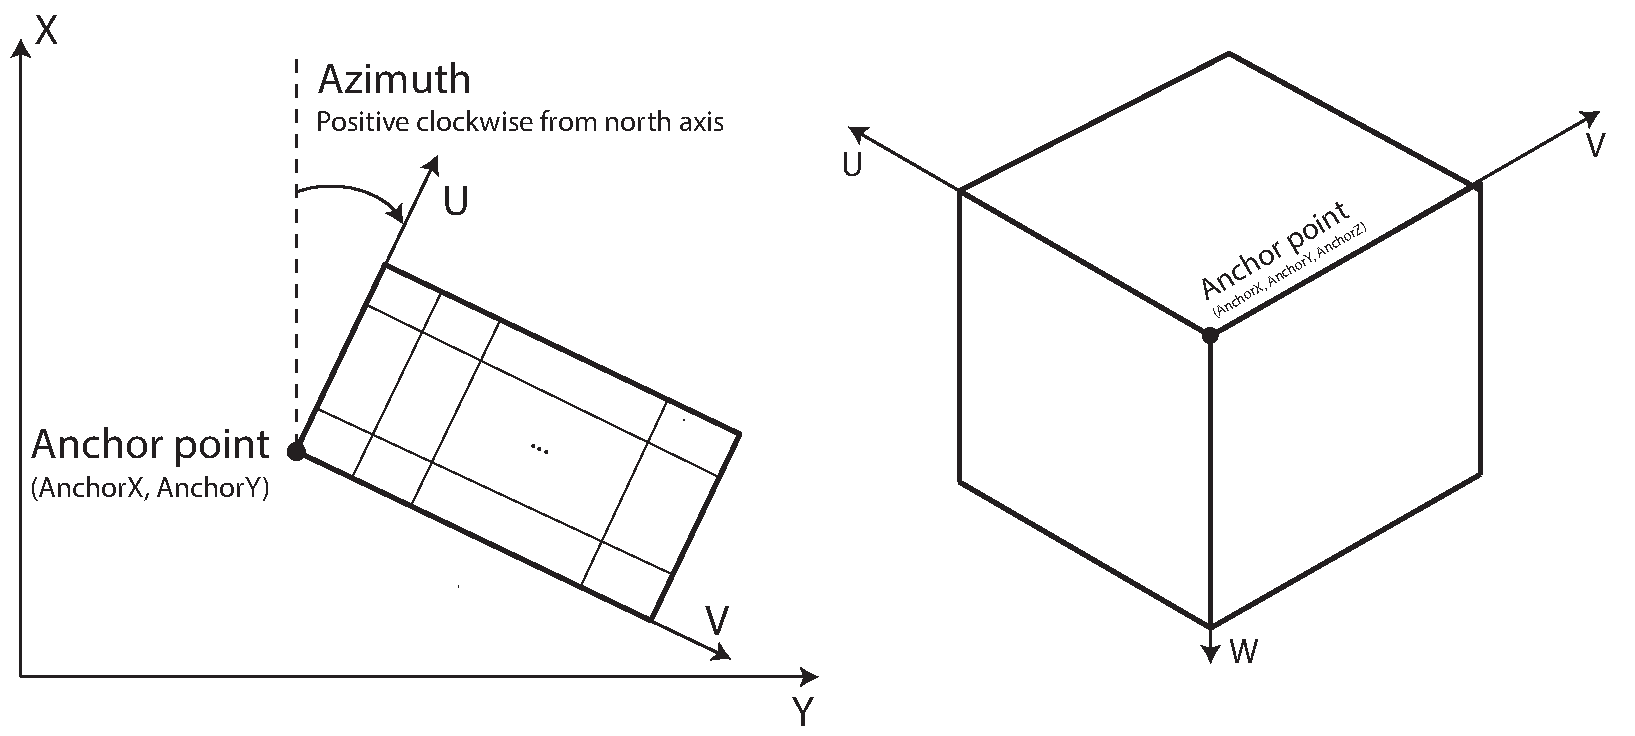
\includegraphics[width=\textwidth]{Figs/reference.pdf}}
\caption{Coordinate system and notation adopted in the format.}
\label{fig:reference}
\end{figure}

The coordinates of the anchor point and the projection type can be specified in the \textit{Georeferencing} group defined in Table \ref{tab:georef}. 

\begin{table}[]
\centering
\caption{Georeferencing group attributes}
\label{tab:georef}
\begin{tabular}{|l|l|l|l|}
\hline
Name & Mandatory & Type & Description \\ \hline
AnchorX & Yes & float64 & Northing of the anchor point \\ \hline
AnchorY & Yes & float64 & Easting of the anchor point \\ \hline
AnchorZ & Yes & float64 & \begin{tabular}[c]{@{}l@{}}Vertical coodinate of the \\ anchor point\end{tabular} \\ \hline
Azimuth & Yes & float64 & \begin{tabular}[c]{@{}l@{}}Azimuth of the model reference \\ frame in degrees\end{tabular} \\ \hline
Projection & No & string & Information about projection. \\ \hline
\end{tabular}
\end{table}

\subsection{Dimensionality}

The format is designed for most general three-dimensional case. Lower dimension models can of course be also stored by ignoring dimensions. For 2D, U is assumed to be the strike direction. Accordingly, for 1D both U and V are ignored.

\section{Structured rectilinear grid}

A mesh is defined by specifying its geometry and physical properties for each cell. This is done via \textit{Geometry} and \textit{Properties} groups as described below. 

\subsection{Geometry group}

The geometry of a rectilinear mesh is uniquely defined by three data sets \textit{NodesU}, \textit{NodesV} and \textit{NodesW} specifying coordinates of the cell nodes in each direction. The sorting of all the arrays is consistent with the orientation of the U,V,W axes, including the storage order of the properties. Group description is given in Tables \ref{tab:geomattr_rect} and \ref{tab:geomdata_rect}.

\begin{table}[]
\centering
\caption{Geometry group attributes}
\label{tab:geomattr_rect}
\begin{tabular}{|l|l|l|l|}
\hline
Name & Mandatory & Type & Description \\ \hline
NU & Yes & int32 & Number of nodes in U direction \\ \hline
NV & Yes & int32 & Number of nodes in V direction \\ \hline
NW & Yes & int32 & Number of nodes in W direction \\ \hline
\end{tabular}
\end{table}

\begin{table}[]
\centering
\caption{Geometry group data sets}
\label{tab:geomdata_rect}
\begin{tabular}{|l|l|l|l|l|}
\hline
Name & Mandatory & Type & Shape & Description \\ \hline
NodesU & Yes & float64 & NU & Coordinates of nodes in U direction \\ \hline
NodesV & Yes & float64 & NV & Coordinates of nodes in V direction \\ \hline
NodesW & Yes & float64 & NW & Coordinates of nodes in W direction \\ \hline
\end{tabular}
\end{table}

\subsection{Properties group}

Each can be assigned a number of properties. The mandatory properties include a cell type and at least one resistivity value. The group attributes and data sets are given in Tables \ref{tab:propdata_rect} and \ref{tab:propattr_rect}.

\begin{table}[]
\centering
\caption{Properties group data sets}
\label{tab:propdata_rect}
\begin{tabular}{|l|l|l|l|l|}
\hline
Name & Mandatory & Type & Shape & Description \\ \hline
CellType & Yes & int64 & [NU-1, NV-1, NW-1] & Cell type property \\ \hline
Rho & No & float64 & [NU-1, NV-1, NW-1] & Isotropic resistivity \\ \hline
\begin{tabular}[c]{@{}l@{}}RhoV \\RhoH\end{tabular} & No & float64 & [NU-1, NV-1, NW-1] & \begin{tabular}[c]{@{}l@{}}Transversely isotropic \\ resistivity\end{tabular} \\ \hline
\begin{tabular}[c]{@{}l@{}}RhoU \\ RhoV \\ RhoW\end{tabular} & No & float64 & [NU-1, NV-1, NW-1] & Anisotropic resistivity \\ \hline
\begin{tabular}[c]{@{}l@{}}Alpha \\ Beta \\ Gamma\end{tabular} & No & float64 & [NU-1, NV-1, NW-1] & \begin{tabular}[c]{@{}l@{}}Euler angles for general \\ anisotropic resistivity\end{tabular} \\ \hline
\end{tabular}
\end{table}

\begin{table}[]
\centering
\caption{Property dataset attributes}
\label{tab:propattr_rect}
\begin{tabular}{|l|l|l|l|}
\hline
Name & Mandatory & Type & Description \\ \hline
Unit & Yes & string & Physical unit of the property \\ \hline
BlankValue & No & float64 & Blank value identifier. Default is NaN. \\ \hline
\end{tabular}
\end{table}

Cell type property can be used to distinguish air, sea and subsurface or to specify active/inactive inversion domains, etc. 

Cells are counted with respect to U, V and W. For instance, I,J,K=1,1,1 corresponds to the anchor point in the lower-left corner of the model, at the model top point. In this point U=0,V=0,W=0. Indices increase accordingly with U,V,W.

For isotropic models, the resistivity will be specified using the property name of \textsl{Rho}. The resistivity for transversely isotropic model will be specified using the property names of \textit{RhoH} and \textit{RhoV}, while the resistivity for a diagonally anisotropic model will be specified using \textit{RhoU}, \textit{RhoV}, and \textit{RhoW}. Model readers should first query the file for \textit{Rho}, then proceeding to the other levels of anisotropy in ascending order. For the most general case, Euler angles can also be specified.

\subsection{Examples}

In the directory \textit{./examples/rectilinear/} you will find as an example a MATLAB script which writes COMMEMI3D-2 model into HDF5 file with the specified format.

\section{Visualization}

Popular visuzalization software such as Paraview and VisIt support HDF5 format via e\textcolor{red}{X}tended \textcolor{red}{D}ata \textcolor{red}{M}odel \textcolor{red}{F}ormat (XDMF: \textcolor[rgb]{0,0,1}{\underline{www.xdmf.org}}). XDMF uses XML to describe data stored in a HDF5 file. Once XDMF is loaded, the program will refer to the specified HDF5 data sets and read relevant data from them. Due to its simple and intuitive structure, XDMF can be easily generated along with the HDF5 file. An example of an XDMF file that describes COMMEMI3D-2 model stored in the \textit{commemi.h5} file and resulting grid rendered by the Paraview (Figure \ref{fig:commemi}) can be found in the directory \textit{./examples/rectilinear/}.

\begin{figure}
\centerline{\includegraphics[width=\textwidth]{Figs/commemi.png}}
\caption{Cut through the COMMEMI3D-2 model loaded in Paraview with XDMF and HDF5.}
\label{fig:commemi}
\end{figure}

%\section{Unstructured tetrahedral mesh}
%\section{Unstructured hexahedral mesh}
%\section{Non-conforming unstructured hexahedral mesh}

\bibliographystyle{acm}

%\bibliography{refs}

\end{document}
